\documentclass[letterpaper]{article}
\usepackage{spconf,amsmath,amssymb,graphicx}
\usepackage[hidelinks]{hyperref}

\usepackage{subcaption}
\usepackage{tikz}
\usetikzlibrary{arrows.meta}
\usetikzlibrary{positioning}
\usetikzlibrary{arrows}

\usepackage{algorithm}
\usepackage{algpseudocode}

\newcommand{\R}[0]{\mathbb{R}}
\newcommand{\N}[0]{\mathbb{N}}
\newcommand{\C}[0]{\mathbb{C}}
\newcommand{\bigoh}{\mathcal O}

\newcommand{\mypar}[1]{{\bf #1.}}

% TODO: Maybe remove the work efficient and change tree to forest?
\title{Efficient Parallelization of Bor\r{u}vka's Minimum Spanning Tree Algorithm}

\fiveauthors
  {Samuel Anzalone \\[-0.8ex] {\small BS Computational Science} \\[-0.8ex] {\small \texttt{ansamuel@ethz.ch}}}
  {Mike Marti \\[-0.8ex] {\small MS Computer Science} \\[-0.8ex] {\small \texttt{mikmarti@ethz.ch}}}
  {Matteo Kamm \\[-0.8ex] {\small MS Computer Science} \\[-0.8ex] {\small \texttt{matkamm@ethz.ch}}}
  {Hulda L.\ Hannesdóttir \\[-0.8ex] {\small MS Computer Science} \\[-0.8ex] {\small \texttt{hhannesdo@ethz.ch}}}
  {\v{S}imon Hrabec \\[-0.8ex] {\small MS Computer Science} \\[-0.8ex] {\small \texttt{shrabec@ethz.ch}}}

\begin{document}

\maketitle

\begin{abstract}
% Describe in concise words what you do, why you do it (not necessarily
% in this order), and the main result.  The abstract has to be
% self-contained and readable for a person in the general area. You
% should write the abstract last.
\end{abstract}

\section{Introduction}
% Do not start the introduction with the abstract or a slightly modified
% version. It follows a possible structure of the introduction. 
% Note that the structure can be modified, but the
% content should be the same. Introduction and abstract should fill at most the first page, better less.
\label{sec:intro}
In this section we briefly introduce and explain what Minimum-Spanning-Tree algorithms are used for. In addition, we
describe our contribution to the scientific comunity as well as work related to ours.

Formally, an MST of a given undirected connected graph $G = (V, E)$ with vertices $V = \{ 0, \dotsc, n - 1 \}$ and
weighted edges $E \subseteq V \times V$, can be defined as an ayclic subgraph of $G$ which connnects all vertices in
$V$ with the least total weight.

\mypar{Motivation}
% The first task is to motivate what you do.  You can
% start general and zoom in one the specific problem you consider.  In
% the process you should have explained to the reader: what you are doing,
% why you are doing, why it is important (order is usually reversed).
%
% For example, if my result is the fastest sorting implementation ever, one
% could roughly go as follows. First explain why sorting is important
% (used everywhere with a few examples) and why performance matters (large datasets,
% realtime). Then explain that fast implementations are very hard and
% expensive to get (memory hierarchy, vector, parallel). 
%
% Now you state what you do in this paper. In our example: 
% presenting a sorting implementation that is
% faster for some sizes as all the other ones.
The MST problem is one of the most studied problems in combinatorial optimization \cite{graham1985history}. Although the
problem is rather simple, its solutions are often used as part of other algorithms to compute intermediate results.
Other scientific fields, such as epidemiology or taxonomy, apply MST algorithms as can be seen in the following list of
example problems.
\begin{itemize}
  \item \textbf{Networking} MST algorithms find trees in computer networks that can be used for broadcasting without
    loops. % TODO: Maybe cite https://dl.acm.org/doi/10.1145/359657.359665
  \item \textbf{$\frac{3}{2}$-ap\-prox\-i\-mate metric TSP} By combining algorithms that find MSTs, matchings and
    eulerian circuits, one can develop a $\frac{3}{2}$-ap\-prox\-i\-mation algorithm solving the metric traveling
    salesperson problem \cite{christofides1976worst}.
  \item \textbf{Molecular Epidemiology} Minimum-Spanning-Trees are used in molecular epidemiology research to estimate
    relationships among individual strains or isolates \cite{spada2004use, salipante2011inadequacies}.
  \item \textbf{Machine Learning} MSTs are used as part of machine learning algorithms. For example, MSTs can reduce the
    fraction of incorrectly labeled samples when performing brain MRI tissue classification \cite{cocosco2003fully}.
\end{itemize}
For most of these use cases, the speed of the MST algorithm is of great importance e.g. to get quick medical results and
be able to treat the patient accordingly.

\mypar{Contribution}
In our research, we focus on the MST algorithm proposed by Bor\r{u}vka \cite{boruuvka1926jistem, nevsetvril2001otakar},
which is one of the most prominent MST algorithms as of today. We implement this algorithm using different work
distribution and merging strategies. Our implementations use the Message Passing Interface (MPI) for communication.
Randomly generated Kronecker graphs are used to evaluate the performance of our implementation.
% TODO: Mention how we perform compared to other implementations once we have results

\mypar{Related Work}
% Next, you have to give a brief overview of
% related work. For a report like this, anywhere between 2 and 8
% references. Briefly explain what they do. In the end contrast to what
% you do to make now precisely clear what your contribution is.
As the MST problem is very versatile and can be used in various scientific disciplines, there already is some research
on parallelizing MST algorithms. One such paper \cite{chung1996parallel}, which is also the main inspriation of this
project, evaluates how the performance of Bor\r{u}vka behaves when using different pointer jumping schemes. They also
show that in principle a speedup proportional to the number of processors can be achieved.

Other research limits itself on sufficiently dense graphs and presents an algorithm for the bulk synchronous parallel
(BSP) model \cite{dehne1998practical}. Furthermore, a parallelization of the MST algorithm using GPUs is presented in
\cite{de2017parallel}.

Some implementations that can be found make use of wait-free Union-Find data structures \cite{wfuf}. Such data
structures speed-up the merge step of the Vor\r{u}vka algorithm. However, they do not aid in distributing the work over
multiple computing nodes.

Our research is similar to that of Chung and Condon \cite{chung1996parallel}, but differs in the work distribution
strategies applied. Moreover, we also evaluate local merging strategies using Union Find data structures additionaly to
the pointer jumping schemes. We do not, however, use the wait-free implementations of those data structures as described
in \cite{wfuf}.

\section{Background}
% Give a short, self-contained summary of necessary
% background information. For example, assume you present an
% implementation of sorting algorithms. You could organize into sorting
% definition, algorithms considered, and asymptotic runtime statements. The goal of the
% background section is to make the paper self-contained for an audience
% as large as possible. As in every section
% you start with a very brief overview of the section. Here it could be as follows: In this section 
% we formally define the sorting problem we consider and introduce the algorithms we use
% including a cost analysis.
%
% \mypar{Sorting}
% Precisely define sorting problem you consider.
%
% \mypar{Sorting algorithms}
% Explain the algorithm you use including their costs.
%
% As an aside, don't talk about "the complexity of the algorithm.'' It's incorrect,
% problems have a complexity, not algorithms.
\label{sec:background}
In this section we formally introduce the MST problem, as well as Bor\r{u}vka's algorithm and different parallelization
strategies used in our implementations.

\mypar{Spanning Tree/Forest}
A spanning tree (forest) is an acyclic (disconnected) subgraph $T = (V_T, E_T)$ of an undirected graph $G = (V_G, E_G)$,
where $V_T = V_G$ and $E_T \subseteq E_G$. It is easy to see, that a spanning tree for a graph $G$ is not necessarily
unique, i.e. there can be more than one spanning tree of a graph. For instance, the fully connected graph $K_3$ has
three spanning trees. For simplicity, we will use the term spanning tree throughout this report even though we might be
working with spanning forests in case $G$ is not connected.

\mypar{Minimum-Spanning-Tree Problem}
In the MST problem, every edge $e$ of the input graph $G = (V, E)$ has an assoicated weight. Formally, there is a weight
function $w : E \to \N$ that is given as input. The goal is to find a spanning tree with a minimum edge weight sum, i.e.
the edge weight of all other spanning trees is at least as large. Just like with a spanning tree, a MST must not
necessarily be unique for a given graph $G$.

\mypar{Bor\r{u}vka's Algorithm}
Bor\r{u}vka's algorithm \cite{boruuvka1926jistem, nevsetvril2001otakar} solves the MST problem as described above.
Algorithm \ref{alg:boruvka} contains a high-level overview of how the algorithm operates. The algorithm terminates as
soon as $T$ is a spanning tree. In case the input graph is not connected, the termination condition has to be slightly adapted to
arrive at a forest. The sequential runtime is $\bigoh(m \log n)$, where $m = |E|$ and $n = |V|$ of the input graph $G =
(V, E)$.

\begin{algorithm}[!t]
  \caption{Bor\r{u}vka's algorithm}
  \label{alg:boruvka}
  \begin{algorithmic}
    \State $T \gets \{ \}$
    \While{$\exists$ more than one connected component}
      \For{each component $c$ in $T$}
        \State $e \gets$ \Call{FindLightestOutgoingEdge}{$c$}
        \State $T \gets T \cup e$
      \EndFor
      \State \Call{MergeComponents}{}
    \EndWhile
    \State \Return $T$
  \end{algorithmic}
\end{algorithm}

\mypar{Union Find Data structure}
A union-find data structure stores a partition of a set into disjoint subsets in such a way, that finding the
corresponding set of an element and merging two sets takes $\bigoh(\alpha(n))$ time \cite{efficiency_union_find}. These
operations can be used to describe the connected components in the algorithm \ref{alg:boruvka}. Note that the runtime
achieved here is not on a per-operation basis. Single operations can take longer but the data structure adjusts itself
so that successive operations are faster.

We use the so-called path compression strategy when performing \verb|find()| operations and we merge sets by rank during
\verb|union()| calls \cite{intro_to_algos}.

\mypar{Pointer Jumping}
% TODO maybe add a tikz image or algorithm description for this
Pointer jumping \cite{jeje1992introduction} (also referred to as path doubling) is a design technique that allows an
algorithm to follow a path using only logarithmic time with respect to the length of the longest path. It does this by
redirecting the parent pointers that describe the path, to point to the parent of the parent for each vertex on the path
simultaneously. This process is then repeated until every vertex points to the root of the path. This gives a $\bigoh(n
\log n)$ runtime, where $n$ describes the amount of vertices on the path. This is superior to simply iteratively fixing
each vertex individually, which has a potential worst case runtime of $\bigoh(n^2)$.

\mypar{Supervertex Pointer Jumping}
% TODO maybe add a tikz image for this
Supervertex pointer jumping \cite{chung1996parallel} is an extension of pointer jumping that uses randomness to get
achieve an expected linear time algorithm. The technique is best explained in the aformentioned paper, but the high
level idea is to select a set of vertices to be supervertices, perform pointer jumping on all non-supervertices, let each
supervertex point to the next supervertex and repeat the process recursively on the supervertices. After the recursion,
it is sufficient to perform only one more pointer jump for all non-supervertices.

\mypar{MPI}
The message passing interface \cite{clarke1994mpi} is a standard for developing applications on parallel computing
architectures. It defines library routines for inter-core and inter-system communication. Similar to the
C++ standard, there is no reference implementation but multiple open source projects implementing the standard, such as
MPICH and Open MPI \cite{gabriel2004open}.

\mypar{Kronecker Graphs}
Kronecker graphs are a class of graphs constructed from a small base graph by iteratively applying the Kronecker product
\cite{leskovec2010kronecker}. The Graph500, a rating of supercomputer systems focusing on graph algorithms, uses a
variation of this graph construction for their benchmarks \cite{graph500}.

\section{Approach}
\label{sec:approach}
% Now comes the ``beef'' of the report, where you explain what you
% did. Again, organize it in paragraphs with titles. As in every section
% you start with a very brief overview of the section.

% In this section, structure is very important so one can follow the technical content.

% Mention and cite any external resources that you used including libraries or other code.
This section contains information about the different implementations devloped, as well as other technical
details, such as distribution strategies, limitations and the benchmarking infrastructure.

\subsection{Distributing the Work}
There are many ways how a graph can be distributed among multiple computation units. The two strategies that we
identified are distributing the edges and distributing the vertices. A combination of the two would also be conceivable,
but was not considered in this project. As these two strategies have different parallelization capabilities, multiple
implementations for both of these approaches were developed. To get a better understanding of how they operate and how they
compare, the following two paragraphs describe them both.

% TODO maybe move the original input graph into the middle to clearly separate the edge dist. and vertex dist. images
\begin{figure*}
  \begin{subfigure}{0.33\textwidth}
    \centering
    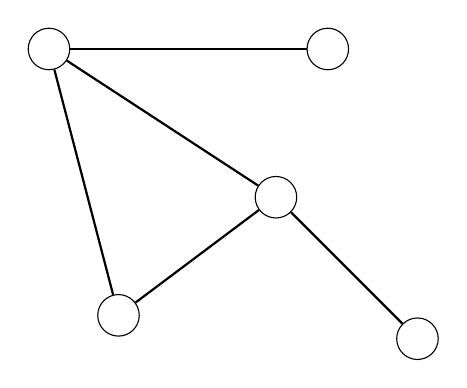
\begin{tikzpicture}[every node/.style={circle,draw,align=center,font=\small,minimum size=1.5em},
      node distance=3cm]
      \node (v1) {};
      \node[below right=3cm and .5cm of v1] (v2) {};
      \node[below right=1.5cm and 2.5cm of v1] (v3) {};
      \node[below right=2cm of v3] (v4) {};
      \node[right=of v1] (v5) {};
      \path[>={Stealth[black]}, every edge/.style={draw=black, thick}]
        (v1) edge (v2)
        (v1) edge (v3)
        (v1) edge (v5)
        (v2) edge (v3)
        (v3) edge (v4);
    \end{tikzpicture}
    \caption{Original input graph}
    \label{fig:work_distribution_original_input_graph}
  \end{subfigure}
  \begin{subfigure}{0.33\textwidth}
    \centering
    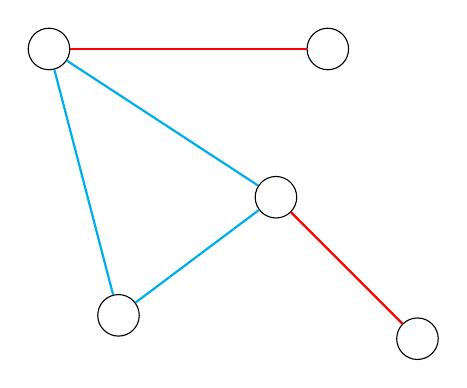
\begin{tikzpicture}[every node/.style={circle,draw,align=center,font=\small,minimum size=1.5em},
      node distance=3cm]
      \node (v1) {};
      \node[below right=3cm and .5cm of v1] (v2) {};
      \node[below right=1.5cm and 2.5cm of v1] (v3) {};
      \node[below right=2cm of v3] (v4) {};
      \node[right=of v1] (v5) {};
      \path[>={Stealth[black]}, every edge/.style={draw=black, thick}]
        (v1) edge[cyan] (v2)
        (v1) edge[cyan] (v3)
        (v1) edge[red] (v5)
        (v2) edge[cyan] (v3)
        (v3) edge[red] (v4);
    \end{tikzpicture}
    \caption{Edge distributed input graph}
    \label{fig:work_distribution_edge_distributed_graph}
  \end{subfigure}
  \begin{subfigure}{0.33\textwidth}
    \centering
    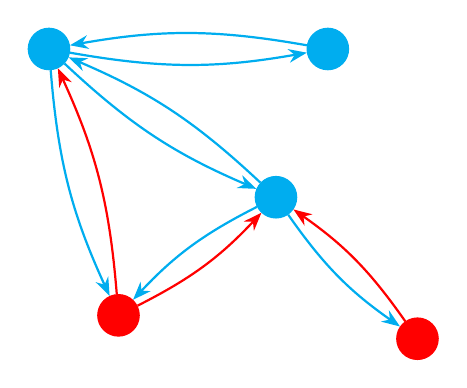
\begin{tikzpicture}[every node/.style={circle,draw,align=center,font=\small,minimum size=1.5em},
      node distance=3cm]
      \node[cyan, fill=cyan] (v1) {};
      \node[red, fill=red, below right=3cm and .5cm of v1] (v2) {};
      \node[cyan, fill=cyan, below right=1.5cm and 2.5cm of v1] (v3) {};
      \node[red, fill=red, below right=2cm of v3] (v4) {};
      \node[cyan, fill=cyan, right=of v1] (v5) {};
      \path[>={Stealth[black]}, every edge/.style={draw=black, thick}]
        [->] [>={Stealth[cyan]}] (v1) edge[cyan, bend right=10] (v2)
        [->] [>={Stealth[red]}] (v2) edge[red, bend right=10] (v1)
        [->] [>={Stealth[cyan]}] (v1) edge[cyan, bend right=10] (v3)
        [->] [>={Stealth[cyan]}] (v3) edge[cyan, bend right=10] (v1)
        [->] [>={Stealth[cyan]}] (v1) edge[cyan, bend right=10] (v5)
        [->] [>={Stealth[cyan]}] (v5) edge[cyan, bend right=10] (v1)
        [->] [>={Stealth[red]}] (v2) edge[red, bend right=10] (v3)
        [->] [>={Stealth[cyan]}] (v3) edge[cyan, bend right=10] (v2)
        [->] [>={Stealth[cyan]}] (v3) edge[cyan, bend right=10] (v4)
        [->] [>={Stealth[red]}] (v4) edge[red, bend right=10] (v3);
    \end{tikzpicture}
    \caption{Vertex distributed input graph}
    \label{fig:work_distribution_vertex_distributed_graph}
  \end{subfigure}
  \caption{Graph distribution example}
  \label{fig:work_distribution}
\end{figure*}

\mypar{Distribution by Edges}
In this approach, the edges of the input graph are distributed evenly among computation units. An illustration of such a
distribution can be seen in Fig. \ref{fig:work_distribution_edge_distributed_graph}. This strategy allows for a uniform
workload distribution, as every computation unit has the same amount of edges to process when selecting the minimum
weight outgoing edges. On the other hand, the merging of components cannot be parallelized using this approach. This is
because during the merging step, all vertices of a component have to unanimously agree on a new leader. But since a
vertex is not owned by a computation unit, this cannot be accomplished without additional effort.

\mypar{Distribution by Vertices}
In this approach, the vertices of the input graph are distrbuted (including their incident edges) among computation
units. An example of such a distribution can be seen in Fig. \ref{fig:work_distribution_vertex_distributed_graph}. One
major disadvantage of this approach is that each edge gets distributed twice because it is not guaranteed that
neighboring vertices are assigned to the same computation unit. Consequently, this strategy requires more time to
distribute the graph. Moreover, the workload of each computation unit is unevenly distributed compared to the edge
distribution strategy. Imagine a scenario, where certain vertices have a higher degree (amount of incident edges) than
others. In that case the computation of the minimum weight outgoing edge of each component takes longer for some
computation units whilst others are idle. However, with this approach the merging of components can be parallelized. 
% TODO: Maybe the last sentence needs more explanation

\subsection{Implementations}
We developed various implementations using C++17, combining different merging approaches with the two aforementioned
distribution strategies. Here is a list of all the combinations that we developed:
\begin{itemize}
  \item Edge distribution using union find data structure
  \item Edge distribution using union find data structure with edge reduction
  \item Edge distribution using pointer jumping
  \item Vertex distribution using union find data structure
  \item Vertex distribution using iterative vertex fixing
  \item Vertex distribution using pointer jumping
  \item Vertex distribution using supervertex pointer jumping
\end{itemize}
As one can see, this list does not contain every possible combination. This is because after some intermediate
benchmarking we focused on the strategies that were the most promising, namely union find and edge distribution.

We are not going to give a detailed description for all of these implementations, as their rough idea should be clear
with the information given in section \ref{sec:background}. The ones that might not be clear are ``edge distribution
using union find data structure with edge reduction'' and ``vertex distribution using iterative vertex fixing''. The first
uses an additional optimization, where edges with endpoints inside the same component get removed once they are
detected. As this removal costs additional runtime, we try to figure out if it is worth the time saved in future
iterations. The second uses an iterative fixing of the vertices, briefly mentioned in the pointer jumping paragraph in
section \ref{sec:background}. This approach has a higher theoretical runtime, but uses far less communication compared
to the pointer jumping strategy. The question was, whether the lower runtime guarantee is worth the additional
communication.

We also implemented sequential versions for some of the merging strategies, to get a better understanding of them.
However, these sequential algorithms did not serve any additional purpose beyond that, i.e. they were not used to get
any measurements.

\mypar{Baseline Implementation}
To get an idea of how well our implementations perform, we decided to use parallel Boost as our baseline. This shows us
how well our implementations hold up against current industry standard code. The reason why we chose parallel Boost is
because it is considered to be the de facto standard when it comes to parallel graph libraries for C++.

\mypar{Kronecker Graph Generator}
We first experimented with different graph types and even implemented some generators for them, but ultimately decided
to only use Kronecker graphs, as they are part of the Graph500 benchmark toolkit to rate supercomputer systems. Compared
to custom generated graphs, the results we get by using Kronecker graphs will be the most unbiased. The generator
implementation that we used is the official Graph500 open source version available on
GitHub\footnote{\url{https://github.com/graph500/graph500/tree/newreference/generator}}, which we copied into our
project and call directly from the source. To get fair and comparable benchmarking results across all algorithm
executions, we seeded the graph generator, such that it always generates the same random graph.

\mypar{Communication}
All implementations use MPI as a communication protocol. Besides send and receive routines used to distribute the
graph, we also use scatter, gather and reduction functionalities in our implementations. To reduce the cost of
communication as far as possible, we kept the amount of MPI subroutine calls to a minimum, by first locally preparing
the data and then sending everything at once.

\mypar{Limitations}
So far all implementations don't compute the actual MST, but only its edge weight sum. In addition, the work has to be
distributed among all computation units evenly, i.e. the amount of edges or vertices must be divisible by the amount of
computation units depending on whether it is an edge or vertex distributed algorithm. For most implementations both of
these limitations would be quite easy to solve. This is especially true for the MST tree computation, as the lightest
edges are distributed among the computation units anyway. However, we disregarded them as being low priority, as our
focus lied on the difference between the various implementation strategies.
% TODO maybe add that it only works with ints so far

\mypar{Correctness}
The correctness of the implementation comes down to the fact that all implementations only terminate once no new edge is
selected, by any computation unit, to the resulting MST. For that reason, the result is a spanning tree. The computed
spanning tree is also a MST due to the greedy nature of how the edges are chosen. The same proof holds as for why the
Bor\r{u}vka's algorithm is correct\cite{nevsetvril2012origins}. For verifying the correctness we use unit tests. We
wrote multiple manual unit tests that cover different edge cases to ensure the correctness of our implementations. On
top of that we also use differential testing with larger Kronocker Graphs (1024 vertices), using the result of the
parallel Boost implementation as a comparison. To get assurance during development and be able to more quickly merge
open pull requests, we used continuous integration to build the application and execute the available unit tests.

\subsection{Benchmarking Infrastructure}
% TODO maybe move likwid description to background -> I think that's unessecary since it doesn't add to any understanding needed for the paper.
To make the experimentation process faster, we developed a small benchmarking infrastructure that allows us to more
easily benchmark the various algorithms with different graph sizes. The measurements were performed using the
performance measurement tool LIKWID \cite{treibig2010likwid}. LIKWID uses hardware counters for its measurements and can
be invoked by putting markers around the code that should be benchmarked. This allowed us to not only benchmark the
entire execution, but also individual parts of the algorithms, which gave us more detailed information about which parts
require the most amount of work.

\section{Experimental Results}\label{sec:exp}

Here you evaluate your work using experiments. You start again with a
very short summary of the section. The typical structure follows.

\mypar{Experimental setup} Specify the platform (processor, frequency, maybe OS, maybe cache sizes)
as well as the compiler, version, and flags used. If your work is about performance, 
I strongly recommend that you play with optimization flags and consider also icc for additional potential speedup.

Then explain what kind of benchmarks you ran. The idea is to give enough information so the experiments are reproducible by somebody else on his or her code.
For sorting you would talk about the input sizes. For a tool that performs NUMA optimization, you would specify the programs you ran.

\mypar{Results}
% TODO compare to results from Chung and Condon
Next divide the experiments into classes, one paragraph for each. In each class of experiments you typically pursue one questions that then is answered by a suitable plot or plots. For example, first you may want to investigate the performance behavior with changing input size, then how your code compares to external benchmarks.

For some tips on benchmarking including how to create a decent viewgraph see pages 22--27 in \cite{Pueschel:10}.

{\bf Comments:}
\begin{itemize}
\item Create very readable, attractive plots (do 1 column, not 2 column plots
for this report) with readable font size. However, the font size should also not be too large; typically it is smaller than the text font size.
An example is in Fig.~\ref{fftperf} (of course you can have a different style).
\item Every plot answers a question. You state this question and extract the
answer from the plot in its discussion.
\item Every plot should be referenced and discussed.
\end{itemize}

\begin{figure}\centering
  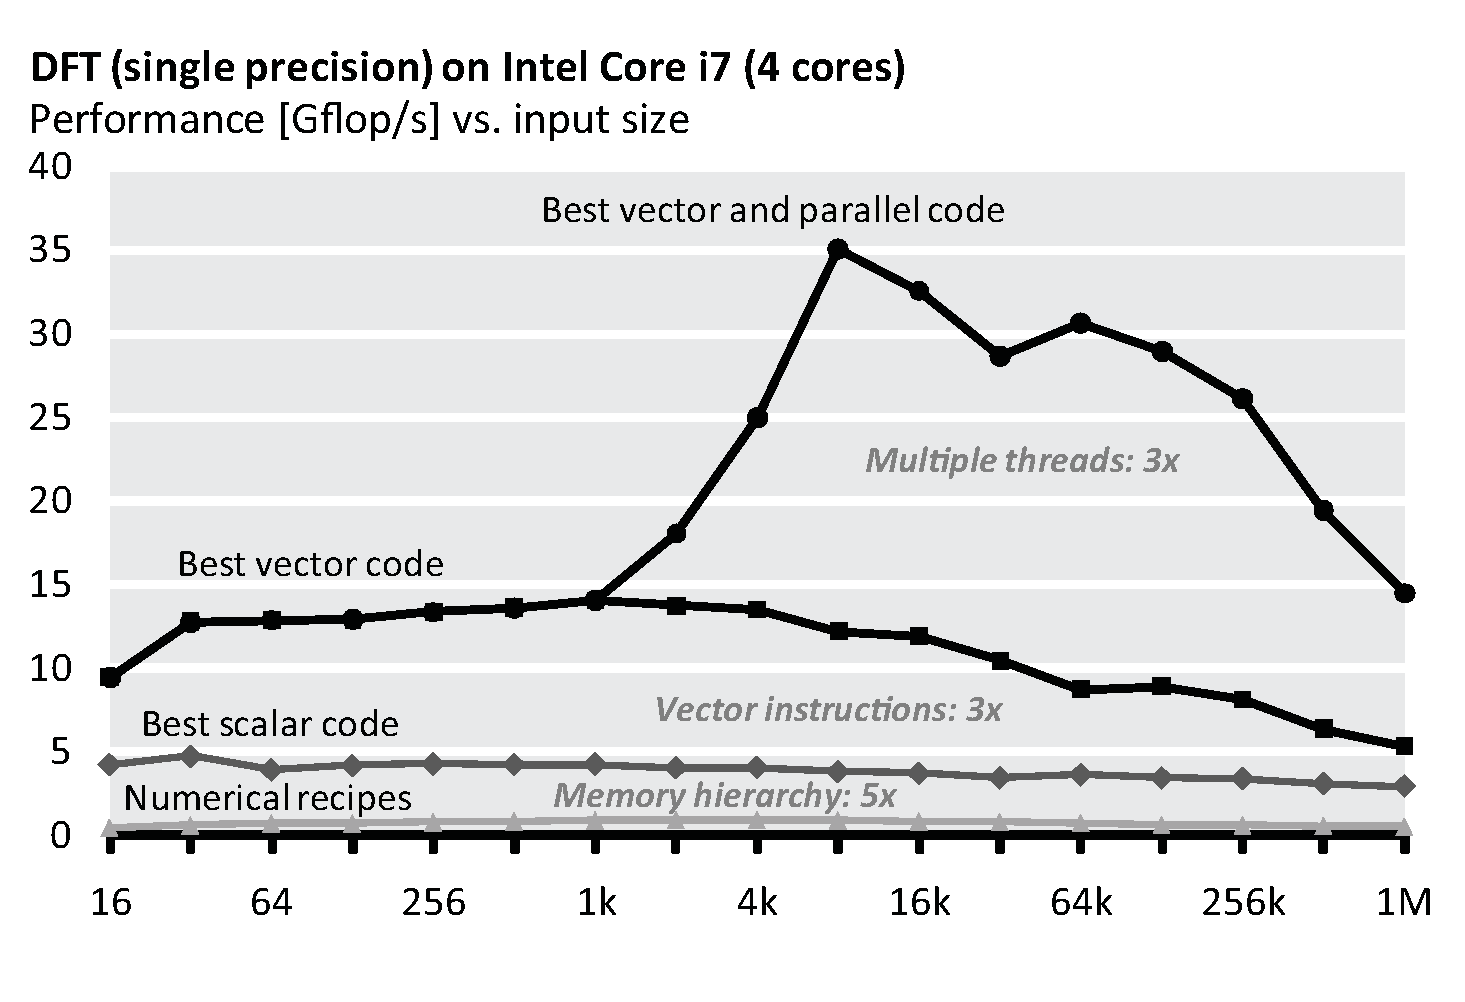
\includegraphics[scale=0.33]{dft-performance.eps}
  \caption{Performance of four single precision implementations of the
  discrete Fourier transform. The operations count is roughly the
  same. The labels in this plot are maybe a little bit too small.\label{fftperf}}
\end{figure}

\section{Conclusions}

Here you need to summarize what you did and why this is
important. {\em Do not take the abstract} and put it in the past
tense. Remember, now the reader has (hopefully) read the report, so it
is a very different situation from the abstract. Try to highlight
important results and say the things you really want to get across
such as high-level statements (e.g., we believe that .... is the right
approach to .... Even though we only considered x, the
.... technique should be applicable ....) You can also formulate next
steps if you want. Be brief. After the conclusions there are only the references.

\section{Further comments}

Here we provide some further tips.

\mypar{Further general guidelines}

\begin{itemize}
\item For short papers, to save space, I use paragraph titles instead of
subsections, as shown in the introduction.

\item It is generally a good idea to break sections into such smaller
units for readability and since it helps you to (visually) structure the story.

\item The above section titles should be adapted to more precisely
reflect what you do.

\item Each section should be started with a very
short summary of what the reader can expect in this section. Nothing
more awkward as when the story starts and one does not know what the
direction is or the goal.

\item Make sure you define every acronym you use, no matter how
convinced you are the reader knows it.

\item Always spell-check before you submit (to us in this case).

\item Be picky. When writing a paper you should always strive for very
high quality. Many people may read it and the quality makes a big difference.
In this class, the quality is part of the grade.

\item Books helping you to write better: \cite{Higham:98} and \cite{Strunk:00}.

\item Conversion to pdf (latex users only): 

dvips -o conference.ps -t letter -Ppdf -G0 conference.dvi

and then

ps2pdf conference.ps
\end{itemize}

\mypar{Graphics} For plots that are not images {\em never} generate the bitmap formats
jpeg, gif, bmp, tif. Use eps, which means encapsulate postscript. It is
scalable since it is a vector graphic description of your graph. E.g.,
from Matlab, you can export to eps.

The format pdf is also fine for plots (you need pdflatex then), but only if the plot was never before in the format 
jpeg, gif, bmp, tif.

\bibliographystyle{IEEEbib}
\bibliography{bibl_conf}

\end{document}

